%\vspace{-0.05in}
\section{Motivation and Background}
\label{background}
%\vspace{-0.05in}

\subsection{{Heterogeneous CC-NUMA Systems}}
\label{heterogeneous_background}
%\vspace{-0.05in}
Systems using heterogeneous CPU and GPU computing resources
have been widely used for several years.  Until recently, the GPU 
has been managed as a separate accelerator, requiring 
explicit memory management by the programmer to transfer data to and 
from the GPU's address space and (typically) the GPU's locally-attached
memory.  To increase programmer productivity and broaden the classes
of workloads that the GPU can execute, recent systems have introduced
automatic memory management enabling the CPU and GPU to access a unified
address space and transparently migrate data at a page-level 
granularity~\cite{UVM}.
The next step in this evolution is making the GPU a cache-coherent peer
to the CPU in the memory system, which is the stated goal of a number
of commercial vendors~\cite{HSA}.

\begin{figure}[t]
    \subfloat[Bandwidth sensitivity] {
        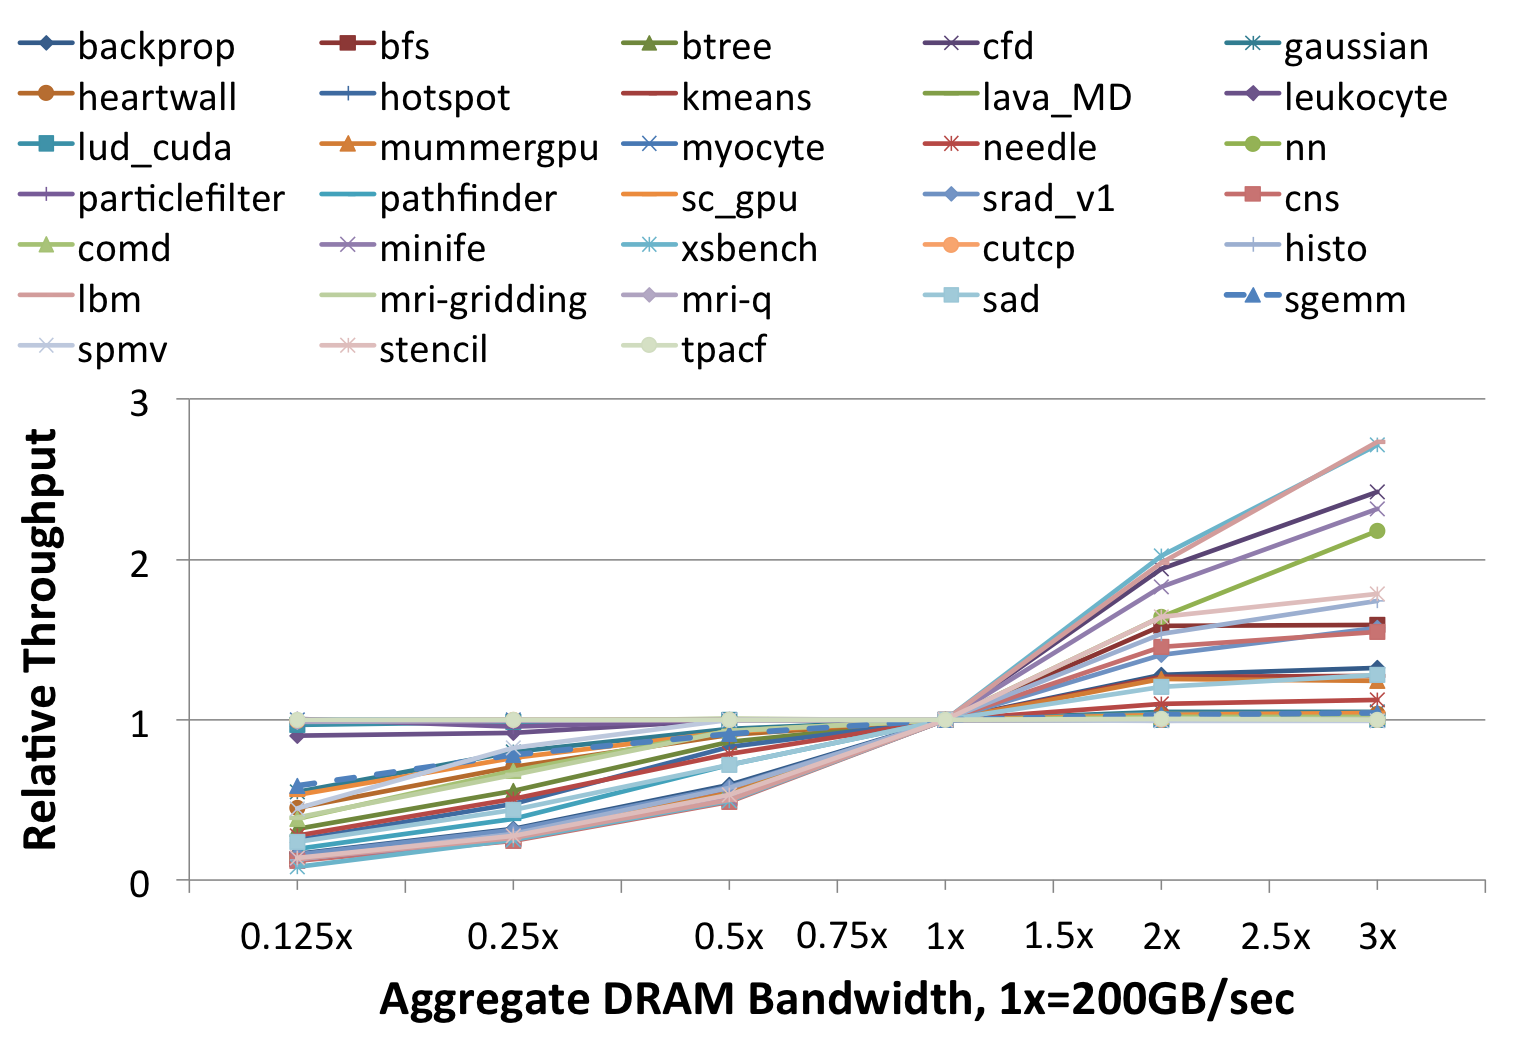
\includegraphics[width=\columnwidth]{asplos2015/figures/bandwidth-1.png}
        \label{fig:bandwidth}
    }
    \\
    \subfloat[Latency sensitivity] {
        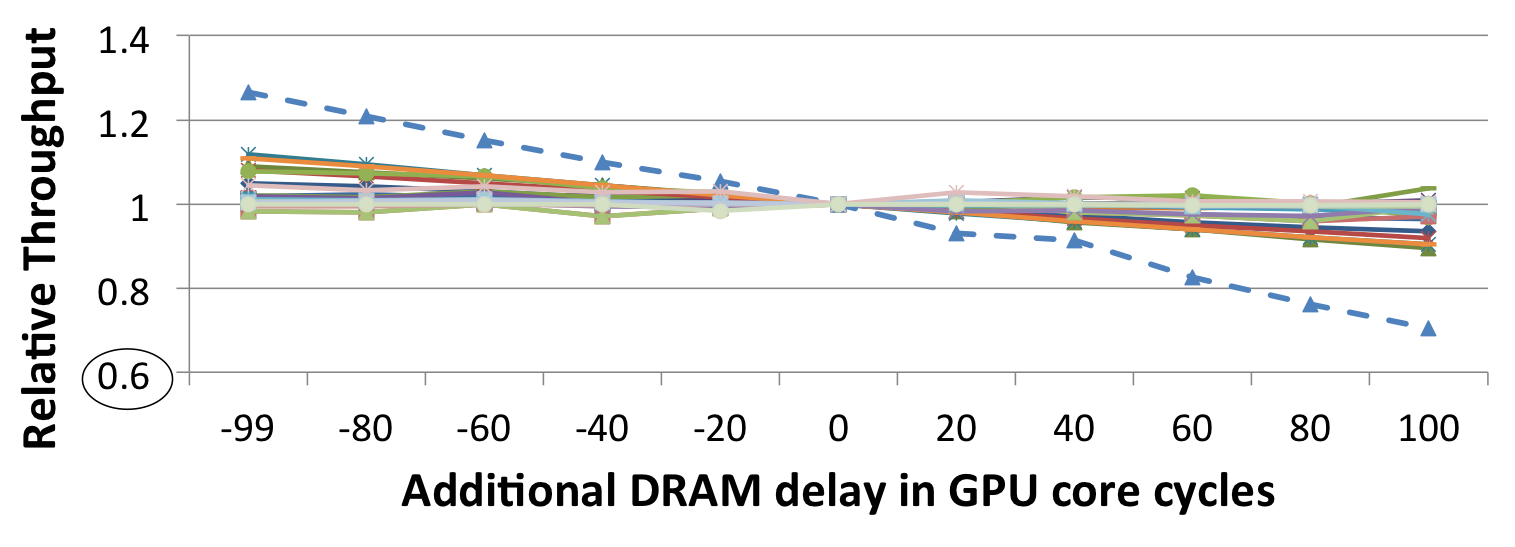
\includegraphics[width=\columnwidth]{asplos2015/figures/latency-1.png}
        \label{fig:latency}
    }
    \caption{GPU performance sensitivity to bandwidth and latency changes.}
    \label{fig:bwlatencysensitivity}
\end{figure}

While some heterogeneous CPU/GPU systems share a single unified physical memory~\cite{AMDAPU},
discrete GPUs are already using specialized DRAM optimized to meet their high bandwidth demands.  
To highlight the sensitivity of GPU performance to memory characteristics, Figures~\ref{fig:bandwidth} and~\ref{fig:latency} show the
performance variation as memory bandwidth and latency vary for a variety of GPU compute benchmarks from the
Rodinia~\cite{Che2009} and {\color{black}Parboil~\cite{Parboil} suites, as well as a number of recent HPC~\cite{comd,cns,minife,xsbench}
workloads. Most of these GPU workloads are
sensitive to changes in bandwidth, while showing much more modest
sensitivity to varying the latency; only {\tt sgemm} stands
out as highly latency sensitive among these 33 workloads. Some application kernels are
neither bandwidth nor latency sensitive and do not see significant performance variation
as modifications are made to the memory subsystem.} While GPU-equipped systems generally require bandwidth-optimized memories to achieve peak performance,
these memory technologies have significant cost, capacity, and/or energy disadvantages over alternative DRAM technologies.

The most common bandwidth-optimized (BO) memory technology today is GDDR5~\cite{GDDR5}.  Providing a per-pin
data rate of up to 7Gbps, this memory technology is widely used with discrete GPUs used in HPC,
workstation, and desktop systems.  Due to the high data rates, GDDR5 systems require significant energy per access
and are unable to support high-capacity multi-rank systems.
In contrast, the roadmap for the next several years of cost/capacity-optimized (CO) DRAM (DDR4 and LPDDR4) 
provides a per-pin data rate that reaches only 3.2 Gbps.  However, these CO DRAM technologies provide similar latency at 
a fraction of the cost and lower energy per access compared to the BO GDDR5 memories.
Looking forward, systems requiring more bandwidth and/or reduced energy per access are moving to  
die-stacked DRAM technologies~\cite{HBM,WIDEIO2}.  These bandwidth-optimized stacked memories are 
significantly more energy-efficient than off-package memory technologies like GDDR5, DDR4, and LPDDR4.  
Unfortunately, the number of DRAM die that can be economically stacked in a single package is limited, 
necessitating systems to also provide a pool of off-package capacity-optimized DRAM.

This disaggregation of memory into on-package and off-package pools is one factor motivating
the need to revisit page placement within the context of GPU performance.  Future GPU/CPU systems are 
likely to take this disaggregation further and move capacity-optimized memory not 
just off the GPU package, but across a high speed interconnect where it is physically attached to the CPU
rather than the GPU, or possibly further~\cite{limchang09}.  
In a CC-NUMA system, the physical location of this capacity-optimized memory only changes the latency and bandwidth
properties of this memory pool -- it is functionally equivalent regardless of being CPU or GPU locally attached.  A robust
page placement policy for GPUs will abstract the on-package, off-package, and remote memory properties into
performance and power characteristics based on which it can make optimized decisions.

\subsection{Current OS NUMA Page Placement}
\label{linux_background}
%\vspace{-0.05in}
In modern symmetric multiprocessor (SMP) systems, each socket typically
consists of several {\color{black}cores} within a chip multi-processor (CMP) that share 
last-level caches and on-chip memory controllers~\cite{INTELXEON}. The number of
memory channels connected to a processor socket is often limited by the
available pin count.  To increase the available memory bandwidth and capacity 
in a system, individual sockets can be connected via a cache coherent interconnect 
fabric such as Intel's Quick Path~\cite{INTELQPI}, AMD's HyperTransport~\cite{AMDHT},
or NVIDIA's NVLink~\cite{NVLINK}.  A single socket, the processors
within it, and the physically attached memory comprise what an operating system
sees as a local NUMA zone.  Each socket is a separate NUMA zone. While a
processor within any given zone can access the DRAM within any other zone, there
is additional latency to service this memory request compared to a locally
serviced memory request because the request must be routed first to its
own memory controller, across the socket interconnect, and through the remote
memory controller.

Operating systems such as Linux have recognized that, unless necessary, it is
typically better for applications to service memory requests from their own
NUMA zone to minimize memory latency.  To get the best performance out of these NUMA
systems, Linux learns system topology information from the Advanced Configuration
and Power Interface (ACPI) System Resource
Affinity Table (SRAT) and memory latency information from the ACPI 
System Locality Information Table (SLIT)\@. After discovering this information,
Linux provides two basic page placement policies that can be specified by 
applications to indicate where they prefer their physical memory pages to be placed
when using standard {\tt malloc} and {\tt mmap} calls to allocate memory.

\emph{LOCAL:} The default policy inherited by user processes is
\emph{LOCAL} in which physical page allocations will be from memory within the 
local NUMA zone of the executing process, unless otherwise specified or due to capacity
limitations.  This typically results in allocations from memory
physically attached to the CPU on which the process is running, thus minimizing
memory access latency.

\emph{INTERLEAVE:} The second available allocation policy, which processes
must specifically inform the OS they would like to use, is \emph{INTERLEAVE}\@. This
policy allocates pages round-robin across all (or a subset)
of the NUMA zones within the SMP system to balance bandwidth across the memory pools.
The downside of this policy is that the additional bandwidth comes at the expense of
increased memory latency. Today, the OS has no knowledge about the relative 
bandwidth of memories in these different NUMA zones because SMP
systems have traditionally had bandwidth-symmetric memory systems.

In addition to these OS placement policies, Linux provides a library interface called \textit{libNUMA}
for applications to request memory allocations from
specific NUMA zones.  This facility provides low-level control over memory placement
but requires careful programming because applications running on different systems will often have
different NUMA-zone layouts.  Additional difficulties arise because there is no performance
feedback mechanism available to programmers when making memory placement decisions, nor are they
aware of which processor(s) their application will be running on while writing their application.

With the advent of heterogeneous memory systems, the assumptions
that operating system NUMA zones will be symmetric in bandwidth, latency, and power characteristics break down.  
The addition of heterogeneous GPU and CPU computing resources further stresses the page placement
policies since processes may not necessarily be migrated to help 
mitigate performance imbalance, as 
certain phases of computation are now pinned to the type of processor executing the program.
As a result, data placement policies combined with bandwidth-asymmetric
memories can have significant impact on GPU, and possibly CPU, performance.

% move related work up to the background and motivation
\subsection{Related Work}
\label{related_work}
%\vspace{-0.05in}
With the introduction of symmetric multiprocessors, significant work has examined optimal placement of processes and memory
in CC-NUMA systems~\cite{Wilson2001,Bolosky1989,Brecht1993,LaRowe1992,Verghese1996,Iyer1998}.
While much of this early work focused on placing processes and data in
close proximity to each other,  more recent work has recognized that
sharing patterns, interconnect congestion, and even queuing
delay within the memory controller are important metrics to consider when
designing page and process placement policies~\cite{AUTONUMA,Dashti2013,Tam2007,Zhuravlev2010,Knauerhase2008,Blagodurov2011,awasthinellans10}.
Nearly all of these works focus on improving traditional CPU throughput
where reduced memory latency is the primary driver of memory system performance.
Recent work from Gerofi et al.~\cite{Gerofi2014} examines TLB replacement policies for the Xeon Phi
co-processor with a focus on highly parallel applications with large data
footprints.

Using non-DRAM technologies or mixed DRAM technologies for main memory systems to improve power
consumption on traditional CPUs has also been
explored by several groups~\cite{Kultursay2013,Phadke11mlpaware2011,Mogul2009,Bheda2011,Ramos2011,Nil2012,pavlovic2013}.  
Much of this work has focused on overcoming the performance
peculiarities that future non-volatile memory (NVM) technologies may have compared to existing DRAM designs.
In addition to mixed technology off-package memories, upcoming on-package memories provide opportunities
for latency reduction by increasing the number of banks available to the application~\cite{Dong2010}
and may one day be configurable to balance bandwidth application needs with power
consumption~\cite{Zhao2012}.
An alternative to treating heterogeneous memory systems as a flat
memory space is to use one technology as a cache for the other~\cite{jiang2011,Meza2012}.  While this
approach has the advantage of being transparent to the programmer, 
{\color{black}OS, and runtime systems}, 
few implementations~\cite{Sim2012} take advantage of the additive bandwidth available
when using heterogeneous memory.

In the GPU space, Zhao et al.~\cite{zhao2013} have explored the affect 
of hybrid DRAM-NVM systems on GPU compute workloads, making the observation that modern GPU designs are very
good at hiding variable memory system latency. Wang et al.~\cite{Wang2013} explore a mixed NVM-DRAM
system that uses compiler analysis to identify near-optimal data placement across kernel invocations
for their heterogeneous memory system. While their system 
does not significantly improve performance, it offers improved power 
efficiency through use of NVM memory and shows that software based page 
placement, rather than hardware caching, can be a viable 
alternative to managing heterogeneous memory for use with GPUs.

